\documentclass{beamer}


%------------------------------------------------
% Tema e configurações
%------------------------------------------------

\usetheme{Madrid}

% Remove barra superior e inferior
\setbeamertemplate{headline}{}
\setbeamertemplate{footline}{}


%------------------------------------------------
% Pacotes
%------------------------------------------------

\usepackage[utf8]{inputenc}
\usepackage[T1]{fontenc}
\usepackage{graphicx}
\usepackage{xcolor}
\usepackage{tikz}
\usepackage{booktabs}

% Imagens: logos nesta pasta e gráficos gerados pelo código
\graphicspath{{./}{../resultados/}}


%------------------------------------------------
% Cores UFT
%------------------------------------------------

\definecolor{uftverde}{RGB}{0,120,100}
\definecolor{uftamarelo}{RGB}{240,180,20}
\definecolor{uftazul}{RGB}{0,80,120}


\setbeamercolor{structure}{fg=uftverde}

\setbeamercolor{frametitle}{
bg=uftverde,
fg=white
}


\setbeamercolor{title}{
fg=uftverde
}


%------------------------------------------------
% Informações
%------------------------------------------------

\title{
Q-Learning no CliffWalking
}


\subtitle{
Aprendizado por Reforço no Planejamento de Trajetória
}


\author{
Lucas Monteiro de Carvalho
}


\institute{
Universidade Federal do Tocantins\\
Curso de Ciência da Computação
}


\date{
2026
}


\setbeamertemplate{footline}{
    \hfill
    \insertframenumber/\inserttotalframenumber
    \hspace{0.5cm}
    \vspace{0.2cm}
}
%------------------------------------------------
\begin{document}
%------------------------------------------------



%================================================
% CAPA
%================================================

\begin{frame}


\begin{tikzpicture}[remember picture,overlay]


% Logo UFT inferior esquerdo

\node[
anchor=south west,
xshift=1.1cm,
yshift=0.5cm
]
at (current page.south west)
{

\includegraphics[height=1.1cm]{Logo_UFT.jpeg}
};



% Logo Ciência da Computação ao lado

\node[
anchor=south west,
xshift=2.5cm,
yshift=0.5cm
]
at (current page.south west)
{

\includegraphics[height=1.1cm]{images.png}
};



\end{tikzpicture}



\vspace{1cm}



\begin{center}



% Título

{\Large
\textcolor{uftverde}{
\textbf{
APRENDIZADO POR REFORÇO\\
COM Q-LEARNING
}
}
}



\vspace{0.4cm}



{\normalsize
Aprendizado por Reforço no Planejamento de Trajetória
}



\vspace{1cm}



{\large
Lucas Monteiro de Carvalho
}



\vspace{0.5cm}



\textbf{
Ciência da Computação
}



\vspace{0.2cm}


Universidade Federal do Tocantins



\vspace{0.8cm}



2026



\end{center}


\end{frame}




%================================================
% SLIDE 2
%================================================


\begin{frame}

\frametitle{O problema}



\textbf{Objetivo:} um agente deve aprender, por tentativa e erro,
o melhor caminho de \textbf{S} até \textbf{G} sem cair no penhasco.



\vspace{0.3cm}



\begin{center}
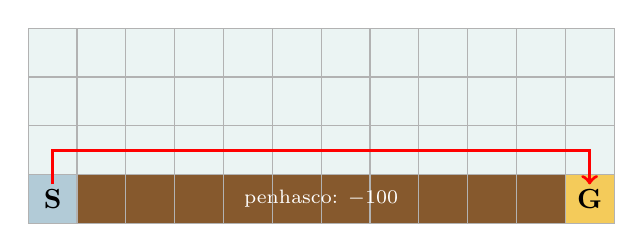
\begin{tikzpicture}[x=0.62cm, y=0.62cm]
\foreach \c in {0,...,11}
  \foreach \l in {1,2,3}
    \draw[gray!60, fill=uftverde!8] (\c,\l) rectangle ++(1,1);
\foreach \c in {1,...,10}
  \draw[gray!60, fill=brown!70!black] (\c,0) rectangle ++(1,1);
\draw[gray!60, fill=uftazul!30] (0,0) rectangle ++(1,1);
\draw[gray!60, fill=uftamarelo!70] (11,0) rectangle ++(1,1);
\node at (0.5,0.5) {\textbf{S}};
\node at (11.5,0.5) {\textbf{G}};
\node[white, font=\scriptsize] at (6,0.5) {penhasco: $-100$};
\draw[red, very thick, ->] (0.5,0.8) -- (0.5,1.5) -- (11.5,1.5) -- (11.5,0.8);
\end{tikzpicture}
\end{center}



\vspace{0.2cm}



\begin{itemize}

\item \textbf{Ambiente:} CliffWalking-v1 (Gymnasium) -- grade $4 \times 12$;

\item \textbf{Estados:} 48 \quad \textbf{Ações:} 4 (cima, direita, baixo, esquerda);

\item \textbf{Recompensa:} $-1$ por passo e $-100$ ao cair (volta para S).

\end{itemize}



\end{frame}





%================================================
% SLIDE 3
%================================================


\begin{frame}

\frametitle{Como funciona o Q-Learning}



A \textbf{matriz Q} ($48 \times 4$) guarda quanto vale fazer cada ação em cada estado.
Ela começa zerada e, a cada passo, é atualizada por:



\vspace{0.2cm}



\[
Q(s,a) \leftarrow Q(s,a) + \alpha\,\big[\, r + \gamma \max_{a'} Q(s',a') - Q(s,a) \,\big]
\]



\vspace{0.2cm}



\begin{enumerate}

\item escolhe a ação com \textbf{$\varepsilon$-greedy}: 10\% aleatória, 90\% a melhor;

\vspace{0.1cm}

\item executa, recebe a recompensa $r$ e vai para o estado $s'$;

\vspace{0.1cm}

\item atualiza $Q(s,a)$ e repete até chegar em G;

\vspace{0.1cm}

\item treina por \textbf{500 episódios}.

\end{enumerate}



\vspace{0.2cm}



{\small $\alpha = 0{,}1$ (taxa de aprendizado) \quad
$\gamma = 0{,}99$ (desconto) \quad $\varepsilon = 0{,}1$ (exploração)}



\end{frame}





%================================================
% SLIDE 4
%================================================


\begin{frame}

\frametitle{Resultados}



\begin{center}
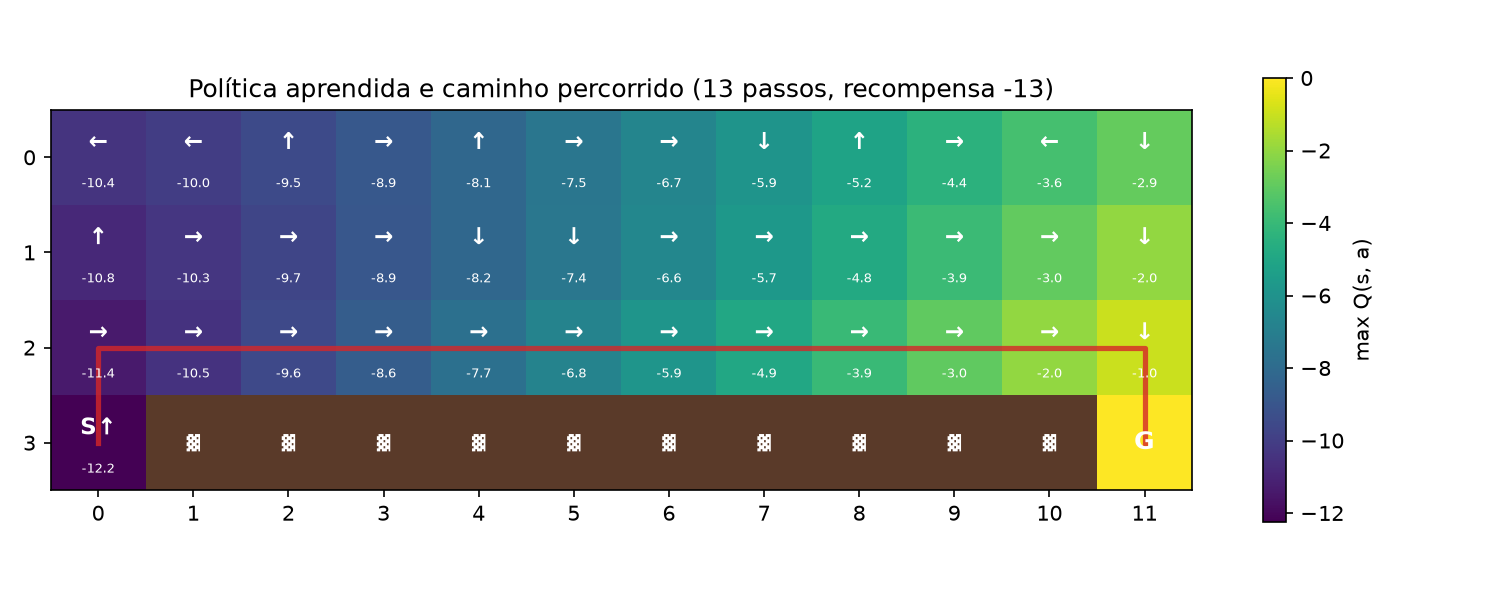
\includegraphics[width=0.95\textwidth]{politica_aprendida.png}
\end{center}



\begin{itemize}

\item a política aprendida chega em G em \textbf{13 passos} (recompensa $-13$), o ótimo;

\vspace{0.1cm}

\item recompensa média: \textbf{$-172$} nos 50 primeiros episódios e \textbf{$-68$} nos 50 últimos;

\vspace{0.1cm}

\item na beira do penhasco, $Q(s,\text{baixo}) \approx -100$: o agente aprendeu a não descer.

\end{itemize}



\end{frame}



%------------------------------------------------

\end{document}
